\section{Headroom Experiment}
\label{sec:headroom}
In this section, headroom experiment results are analyzed to guide our dynamic hybrid prefetcher design. In section \ref{sec:headroomanalysis} we will talk about the potential of our design and the difference between two headroom test. In section \ref{sec:memorybandwidthissue}, one of the most influential factor, memory bandwidth, will be discussed in detail. Some other insights will be revealed in section \ref{sec:otherinsights}.

  \subsection{Headroom Result Analysis}
  \label{sec:headroomanalysis}

  \begin{figure}[ht!]
	   \centering
	   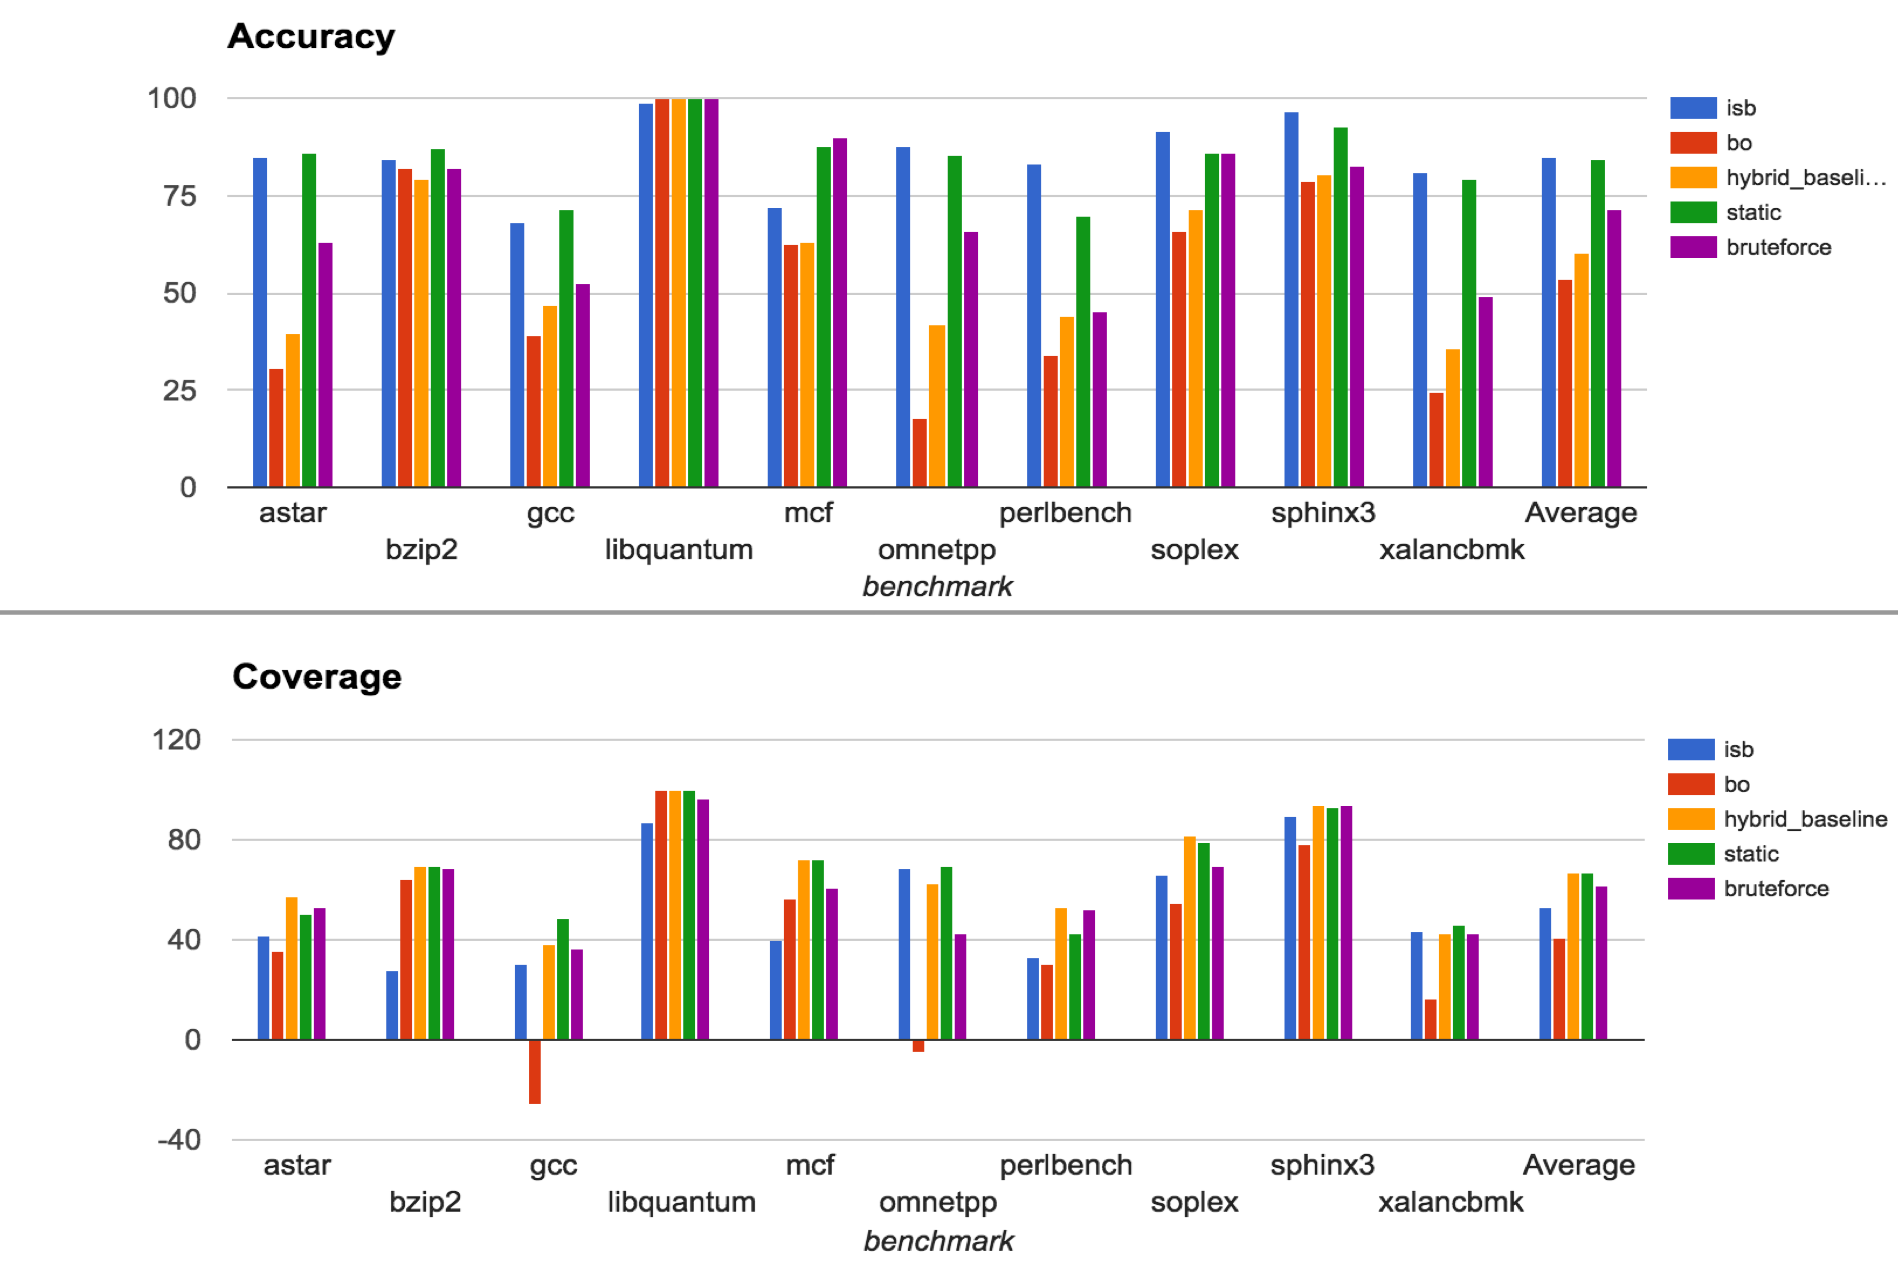
\includegraphics[width=1.0\textwidth]{images/headroom_acc_cov.png}
	   \caption{Headroom accuracy and coverage performance}
	  \label{fig:headroom_acc_cov}
  \end{figure}

  In Fig.\ref{fig:headroom_acc_cov}, the accuracy and coverage performance of \emph{ISB, BO, NHP, Static Analysis} and \emph{Brute Force Search} are shown. Comparing \emph{NHP} with \emph{ISB, BO}, we found that the accuracy of \emph{NHP} is significantly lower than \emph{ISB}'s, while its coverage is higher than \emph{ISB}. It indicates that \emph{NHP} issued much more prefetches than \emph{ISB} and \emph{BO}. For \emph{static analysis} part, it achieves similar accuracy to \emph{ISB}'s, and similar coverage to \emph{NHP}'s. This is understandable since \emph{Static Analysis} focuses on static data files. Making wise decisions is the only thing it can do. The \emph{Brute Force Search} method focuses on speedup most. Therefore, its accuracy and coverage performance are not as good as the static ones'. Note that the accuracy and coverage are the same on 6.4GB/s and 12.8GB/s bandwidth, since prefetching action is not changed different bandwidth.

  Though accuracy and coverage are good metrics for evaluating prefetchers. The most import performance metric is speedup. The speedup numbers of different bandwidth are shown in Fig. \ref{fig:headroom_speedup}. Note that here and in all the later figures, the speedup is comparing to system with no prefetcher. Interestingly, we got results of different shapes when the bandwidth is different. \emph{ISB} has higher speedup on low bandwidth while \emph{BO} has higher on high bandwidth. The reason is that high bandwidth wouldn't give much punishment to useless prefetches while low bandwidth does. For \emph{NHP}, in both configuration it enjoys higher speedup. However, the headroom of 6.4GB/s bandwidth is more than 11\%, while only 4\% in 12.8GB/s bandwidth case. Another point worth attention is that though static method enjoys higher accuracy and coverage than the brute force one, \emph{Brute Force Search} still has better speed up. Intuitively, it is because some prefetches shouldn't have been issued by \emph{Static Analysis} due to high memory pressure at that point. The detail reason will be explained in section \ref{sec:memorybandwidthissue}.

  In our later evaluation, we will choose 6.4GB/s as our bandwidth since the headroom is quite encouraging in that case.

  %higher accuracy and coverage doesn't imply better speedup.

  \begin{figure}[ht!]
	   \centering
	   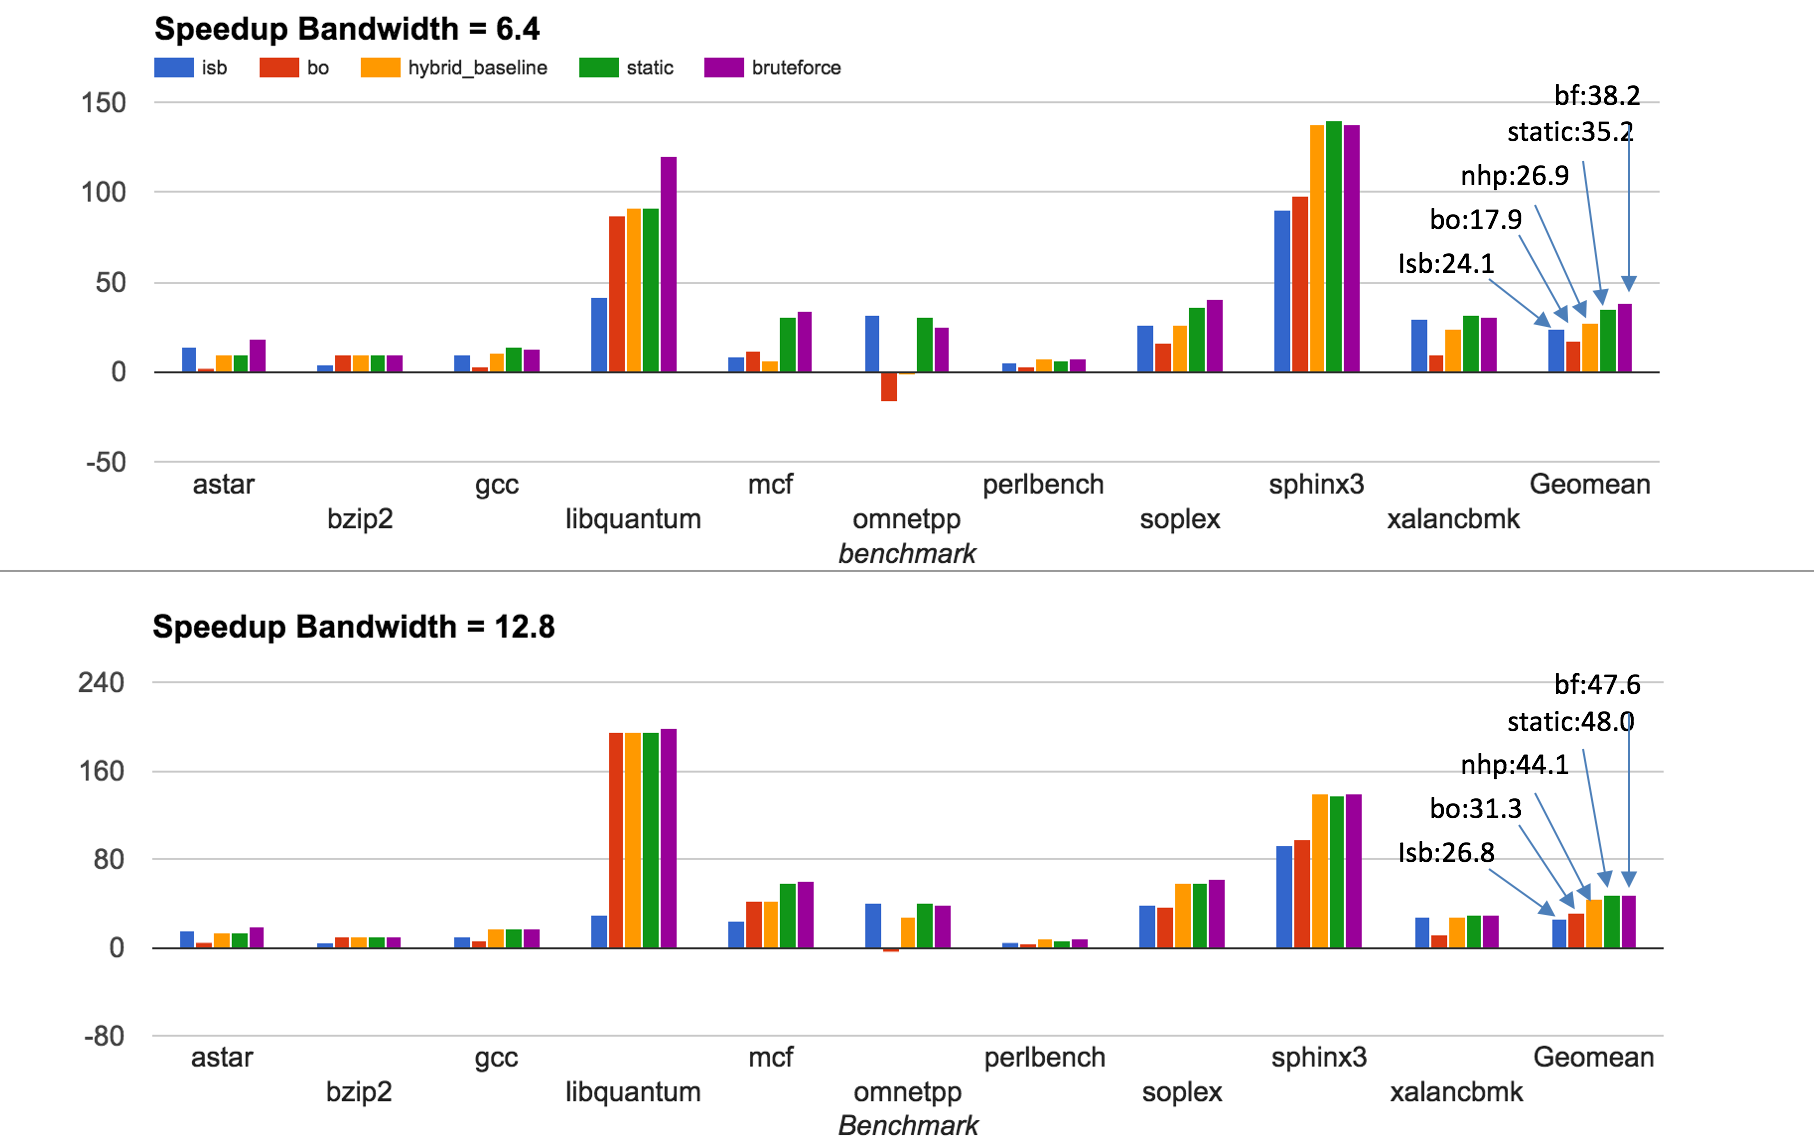
\includegraphics[width=1.0\textwidth]{images/headroom_speedup.png}
	   \caption{Headroom speedup under different memory bandwidth}
	  \label{fig:headroom_speedup}
  \end{figure}

  \subsection{Memory Bandwidth Issue}

  \label{sec:memorybandwidthissue}
  Fig. \ref{fig:headroom_speedup} shows that the headroom of hybrid prefetching system is highly related to memory bandwidth, and it is consistent with our previous discussion: hybrid prefetching system is limited by the amount of shared resources. 
  The less resources it has, the more headroom it can achieve.\par
  In this part we will discuss in detail how the memory bandwidth influences our performance, and how we can deal with it.\par
  

    \begin{figure}[h]
	   \centering
	   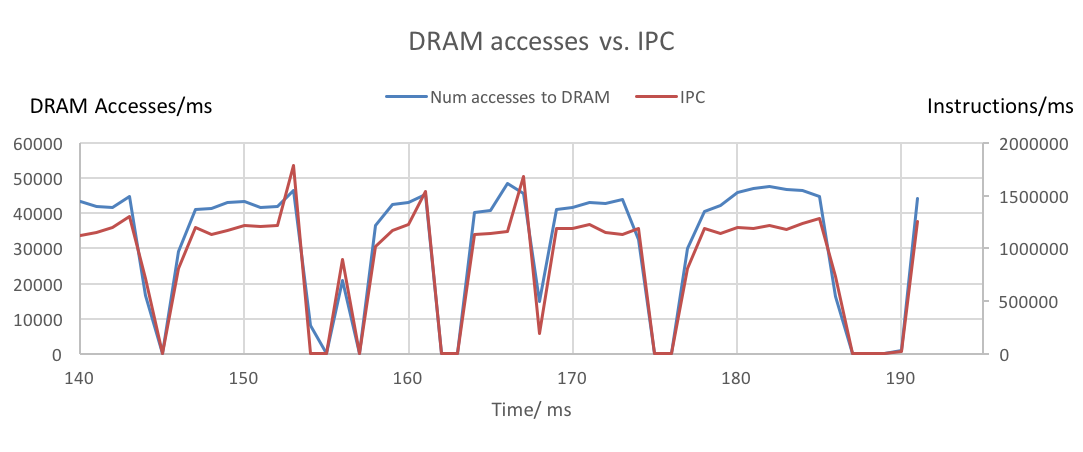
\includegraphics[width=0.8\textwidth]{images/bandwidth_IPC.png}
	   \caption{DRAM accesses vs IPC}
	  \label{fig:bandwidth_IPC}
  \end{figure}
  \begin{figure}[h]
	   \centering
	   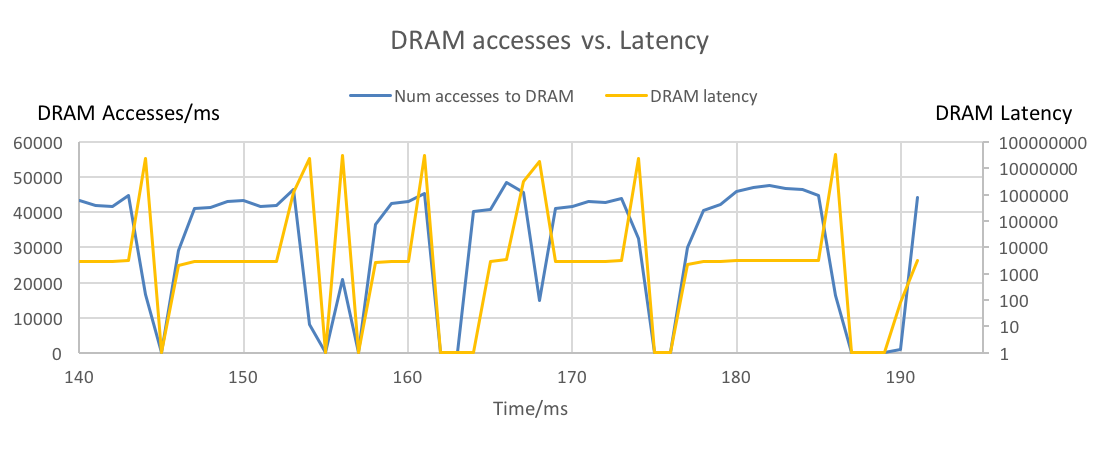
\includegraphics[width=0.8\textwidth]{images/bandwidth_latency.png}
	   \caption{DRAM accesses vs DRAM latency}
	  \label{fig:bandwidth_latency}
  \end{figure}

Fig. \ref{fig:bandwidth_IPC} and Fig. \ref{fig:bandwidth_latency} show bandwidth, IPC and memory latency from benchmark \emph{astar} sim point 1 from 140ms to 192ms. The blue lines in both graphs are numbers of DRAM accesses per ms, which denotes the bandwidth usage. Red line is the number of executed instructions per ms, which denotes IPC. Yellow line is the sum of latency of all DRAM accesses per ms. X axis is the time line.\par
In Fig. \ref{fig:bandwidth_IPC}, DRAM accesses and IPC almost overlap. This indicates that at the low points, the benchmark program is stalled and DRAM doesn't receive any more request. For those low points in Fig. \ref{fig:bandwidth_latency}, latency increases a lot at the low points. Note that the latency Y axis is in log scale, the latency actually increases four to five magnitudes at those moments. The reason why the peak points of yellow is a little before the low points of blue is that, the sniper simulator calculates the latency of an access at the moment it is issued, not at the moment it returns.\par
 We can draw conclusions from these two figures that: 1) On some benchmarks, programs are occasionally stalled due to limited memory bandwidth and this is a significant issue to the performance. 2) Memory bandwidth should be considered in the hybrid prefetching system.  In our current headroom experiments, PCs make static decisions offline and never change decisions during execution. When we implement dynamic hybrid system, bandwidth usage is a factor to control the prefetching degree of prefetchers. \par


  \subsection{Some other insights}
  \label{sec:otherinsights}
  Besides memory bandwidth factor, we have some other insights about these headroom experiments.
  \begin{itemize}
    \item Performance is input dependent. A well built benchmark set is important
    \item The brute force experiments are not optimal, but they can still show the preference of each PC.
    \item In the headroom experiment, PCs’ decisions are made offline and not changed during execution. And we have up to 12\% speedup headroom. If PC can make dynamic decisions, we may have more speedup.
    \item Memory bandwidth pressure affects the prefetch performance a lot. It needs to be considered and measured in dynamic hybrid prefetching system.
  \end{itemize}
